% Options for packages loaded elsewhere
\PassOptionsToPackage{unicode}{hyperref}
\PassOptionsToPackage{hyphens}{url}
\PassOptionsToPackage{dvipsnames,svgnames,x11names}{xcolor}
%
\documentclass[
  10pt,
]{article}
\usepackage{amsmath,amssymb}
\usepackage{iftex}
\ifPDFTeX
  \usepackage[T1]{fontenc}
  \usepackage[utf8]{inputenc}
  \usepackage{textcomp} % provide euro and other symbols
\else % if luatex or xetex
  \usepackage{unicode-math} % this also loads fontspec
  \defaultfontfeatures{Scale=MatchLowercase}
  \defaultfontfeatures[\rmfamily]{Ligatures=TeX,Scale=1}
\fi
\usepackage{lmodern}
\ifPDFTeX\else
  % xetex/luatex font selection
  \setmainfont[]{DejaVu Serif}
  \setmonofont[]{DejaVu Sans Mono}
\fi
% Use upquote if available, for straight quotes in verbatim environments
\IfFileExists{upquote.sty}{\usepackage{upquote}}{}
\IfFileExists{microtype.sty}{% use microtype if available
  \usepackage[]{microtype}
  \UseMicrotypeSet[protrusion]{basicmath} % disable protrusion for tt fonts
}{}
\makeatletter
\@ifundefined{KOMAClassName}{% if non-KOMA class
  \IfFileExists{parskip.sty}{%
    \usepackage{parskip}
  }{% else
    \setlength{\parindent}{0pt}
    \setlength{\parskip}{6pt plus 2pt minus 1pt}}
}{% if KOMA class
  \KOMAoptions{parskip=half}}
\makeatother
\usepackage{xcolor}
\usepackage[margin=0.8in]{geometry}
\usepackage{color}
\usepackage{fancyvrb}
\newcommand{\VerbBar}{|}
\newcommand{\VERB}{\Verb[commandchars=\\\{\}]}
\DefineVerbatimEnvironment{Highlighting}{Verbatim}{commandchars=\\\{\}}
% Add ',fontsize=\small' for more characters per line
\usepackage{framed}
\definecolor{shadecolor}{RGB}{248,248,248}
\newenvironment{Shaded}{\begin{snugshade}}{\end{snugshade}}
\newcommand{\AlertTok}[1]{\textcolor[rgb]{0.94,0.16,0.16}{#1}}
\newcommand{\AnnotationTok}[1]{\textcolor[rgb]{0.56,0.35,0.01}{\textbf{\textit{#1}}}}
\newcommand{\AttributeTok}[1]{\textcolor[rgb]{0.13,0.29,0.53}{#1}}
\newcommand{\BaseNTok}[1]{\textcolor[rgb]{0.00,0.00,0.81}{#1}}
\newcommand{\BuiltInTok}[1]{#1}
\newcommand{\CharTok}[1]{\textcolor[rgb]{0.31,0.60,0.02}{#1}}
\newcommand{\CommentTok}[1]{\textcolor[rgb]{0.56,0.35,0.01}{\textit{#1}}}
\newcommand{\CommentVarTok}[1]{\textcolor[rgb]{0.56,0.35,0.01}{\textbf{\textit{#1}}}}
\newcommand{\ConstantTok}[1]{\textcolor[rgb]{0.56,0.35,0.01}{#1}}
\newcommand{\ControlFlowTok}[1]{\textcolor[rgb]{0.13,0.29,0.53}{\textbf{#1}}}
\newcommand{\DataTypeTok}[1]{\textcolor[rgb]{0.13,0.29,0.53}{#1}}
\newcommand{\DecValTok}[1]{\textcolor[rgb]{0.00,0.00,0.81}{#1}}
\newcommand{\DocumentationTok}[1]{\textcolor[rgb]{0.56,0.35,0.01}{\textbf{\textit{#1}}}}
\newcommand{\ErrorTok}[1]{\textcolor[rgb]{0.64,0.00,0.00}{\textbf{#1}}}
\newcommand{\ExtensionTok}[1]{#1}
\newcommand{\FloatTok}[1]{\textcolor[rgb]{0.00,0.00,0.81}{#1}}
\newcommand{\FunctionTok}[1]{\textcolor[rgb]{0.13,0.29,0.53}{\textbf{#1}}}
\newcommand{\ImportTok}[1]{#1}
\newcommand{\InformationTok}[1]{\textcolor[rgb]{0.56,0.35,0.01}{\textbf{\textit{#1}}}}
\newcommand{\KeywordTok}[1]{\textcolor[rgb]{0.13,0.29,0.53}{\textbf{#1}}}
\newcommand{\NormalTok}[1]{#1}
\newcommand{\OperatorTok}[1]{\textcolor[rgb]{0.81,0.36,0.00}{\textbf{#1}}}
\newcommand{\OtherTok}[1]{\textcolor[rgb]{0.56,0.35,0.01}{#1}}
\newcommand{\PreprocessorTok}[1]{\textcolor[rgb]{0.56,0.35,0.01}{\textit{#1}}}
\newcommand{\RegionMarkerTok}[1]{#1}
\newcommand{\SpecialCharTok}[1]{\textcolor[rgb]{0.81,0.36,0.00}{\textbf{#1}}}
\newcommand{\SpecialStringTok}[1]{\textcolor[rgb]{0.31,0.60,0.02}{#1}}
\newcommand{\StringTok}[1]{\textcolor[rgb]{0.31,0.60,0.02}{#1}}
\newcommand{\VariableTok}[1]{\textcolor[rgb]{0.00,0.00,0.00}{#1}}
\newcommand{\VerbatimStringTok}[1]{\textcolor[rgb]{0.31,0.60,0.02}{#1}}
\newcommand{\WarningTok}[1]{\textcolor[rgb]{0.56,0.35,0.01}{\textbf{\textit{#1}}}}
\usepackage{longtable,booktabs,array}
\usepackage{calc} % for calculating minipage widths
% Correct order of tables after \paragraph or \subparagraph
\usepackage{etoolbox}
\makeatletter
\patchcmd\longtable{\par}{\if@noskipsec\mbox{}\fi\par}{}{}
\makeatother
% Allow footnotes in longtable head/foot
\IfFileExists{footnotehyper.sty}{\usepackage{footnotehyper}}{\usepackage{footnote}}
\makesavenoteenv{longtable}
\usepackage{graphicx}
\makeatletter
\def\maxwidth{\ifdim\Gin@nat@width>\linewidth\linewidth\else\Gin@nat@width\fi}
\def\maxheight{\ifdim\Gin@nat@height>\textheight\textheight\else\Gin@nat@height\fi}
\makeatother
% Scale images if necessary, so that they will not overflow the page
% margins by default, and it is still possible to overwrite the defaults
% using explicit options in \includegraphics[width, height, ...]{}
\setkeys{Gin}{width=\maxwidth,height=\maxheight,keepaspectratio}
% Set default figure placement to htbp
\makeatletter
\def\fps@figure{htbp}
\makeatother
\setlength{\emergencystretch}{3em} % prevent overfull lines
\providecommand{\tightlist}{%
  \setlength{\itemsep}{0pt}\setlength{\parskip}{0pt}}
\setcounter{secnumdepth}{-\maxdimen} % remove section numbering
\ifLuaTeX
  \usepackage{selnolig}  % disable illegal ligatures
\fi
\usepackage{bookmark}
\IfFileExists{xurl.sty}{\usepackage{xurl}}{} % add URL line breaks if available
\urlstyle{same}
\hypersetup{
  colorlinks=true,
  linkcolor={Maroon},
  filecolor={Maroon},
  citecolor={Blue},
  urlcolor={Blue},
  pdfcreator={LaTeX via pandoc}}

\author{}
\date{}

\begin{document}

\section{Simplicial freeze-out: detailed geometry and a guided tour of
the Julia
code}\label{simplicial-freeze-out-detailed-geometry-and-a-guided-tour-of-the-julia-code}

\textbf{Standalone technical notes for a Cartesian spacetime grid}\\
\textbf{Companion source:} \texttt{SimplicialFreezeOut.jl} (fully
commented), \texttt{walkthrough.jl},
\texttt{test\_simplicial\_freezeout.jl}.

\subsection{1. What problem does the code
solve?}\label{what-problem-does-the-code-solve}

We are given a temperature array on a Cartesian-product spacetime grid,

\[
T_{i_0 i_1\cdots i_d}=T(t_{i_0},x^1_{i_1},\ldots,x^d_{i_d}),
\quad D=d+1\in\{2,3,4\}.
\]

We need the codimension-one isothermal set
\(\Sigma=\{X:T(X)=T_{\mathrm{fo}}\}\), together with the oriented
hypersurface elements entering a Cooper--Frye or conserved-current
integral. The algorithm \textbf{does not compute particle spectra}; it
returns a list of small geometric elements and sampled hydrodynamic
fields.

The word \emph{simplex} refers to a spacetime cell used \textbf{to
search for} the surface, not to the surface itself. In \(D\) spacetime
dimensions, the grid cell is decomposed into \(D\)-simplices; their
intersections with the isotherm are \((D-1)\)-dimensional surface
pieces.

\begin{longtable}[]{@{}
  >{\centering\arraybackslash}p{(\columnwidth - 8\tabcolsep) * \real{0.2500}}
  >{\raggedright\arraybackslash}p{(\columnwidth - 8\tabcolsep) * \real{0.1875}}
  >{\raggedright\arraybackslash}p{(\columnwidth - 8\tabcolsep) * \real{0.1875}}
  >{\raggedright\arraybackslash}p{(\columnwidth - 8\tabcolsep) * \real{0.1875}}
  >{\raggedright\arraybackslash}p{(\columnwidth - 8\tabcolsep) * \real{0.1875}}@{}}
\toprule\noalign{}
\begin{minipage}[b]{\linewidth}\centering
Spatial dimensions \(d\)
\end{minipage} & \begin{minipage}[b]{\linewidth}\raggedright
Spacetime coordinates
\end{minipage} & \begin{minipage}[b]{\linewidth}\raggedright
Cartesian spacetime cell
\end{minipage} & \begin{minipage}[b]{\linewidth}\raggedright
Reference decomposition
\end{minipage} & \begin{minipage}[b]{\linewidth}\raggedright
Output surface piece
\end{minipage} \\
\midrule\noalign{}
\endhead
\bottomrule\noalign{}
\endlastfoot
1 & \((t,x)\) & rectangle, 4 corners & 2 triangles, 3 vertices each &
line segment, 2 endpoints \\
2 & \((t,x,y)\) & cube, 8 corners & 6 tetrahedra, 4 vertices each &
triangle, 3 vertices \\
3 & \((t,x,y,z)\) & 4D hypercube, 16 corners & 24 four-simplices, 5
vertices each & tetrahedron, 4 vertices \\
\end{longtable}

A tetrahedron in \((t,x,y)\) is a \textbf{spacetime volume simplex}; a
tetrahedron in \((t,x,y,z)\) is a \textbf{freeze-out hypersurface
element}. These are different roles.

\subsection{2. Two separate decisions, not
one}\label{two-separate-decisions-not-one}

\textbf{Step A: geometrical decomposition.} Every Cartesian cell is cut
into a fixed set of \(D!\) reference simplices, independent of
temperature. We process \textbf{all} of them. There is no question of
selecting one favorite simplex.

\textbf{Step B: temperature-dependent selection.} For each simplex,
examine the signs of \(F_a=T_a-T_{\rm fo}\) at its \(D+1\) vertices. If
all signs agree, the affine temperature inside cannot intersect \(F=0\);
skip it. Otherwise use a precomputed lookup table to identify the
crossing edges and how to connect their intersection points.

At a fixed resolution, this constructs the isotherm of the
\textbf{piecewise-affine reconstructed temperature field}, which need
not coincide exactly with the physical continuum isotherm.

\subsection{3. How the Freudenthal decomposition is
generated}\label{how-the-freudenthal-decomposition-is-generated}

Normalize the coordinate cell to \([0,1]^D\), with coordinates
\(s=(s_1,\ldots,s_D)\) and \(s_1\) representing time. Let \(e_k\) be the
coordinate unit vectors. For each permutation
\(\pi=(\pi_1,\ldots,\pi_D)\), define

\[
V_0=0,\qquad V_j=\sum_{k=1}^{j}e_{\pi_k},\quad j=1,\ldots,D.
\]

The \(D+1\) vertices define one simplex. Each permutation gives one
monotone staircase from \((0,\ldots,0)\) to \((1,\ldots,1)\). The \(D!\)
staircases partition the unit cell without overlapping interiors. They
agree across Cartesian cell faces if every cell uses the same
convention.

The reference vertices are represented by \textbf{bit-coded corner IDs}.
In Julia's one-based indexing, the corner with bits \((b_1,\ldots,b_D)\)
has index

\[
\operatorname{corner}(b)=1+\sum_{\mu=1}^{D}b_\mu 2^{\mu-1}.
\]

Thus in \(D=3\), \(000\mapsto1\), \(100\mapsto2\), \(010\mapsto3\), and
\(111\mapsto8\).

\subsubsection{3.1 Example in one spatial
dimension}\label{example-in-one-spatial-dimension}

The spacetime rectangle \((t,x)\in[0,1]^2\) is cut along the \(00\to11\)
diagonal into

\[
S_1=(00,10,11),\qquad S_2=(00,01,11).
\]

Each triangle can contribute one freeze-out \textbf{segment}.

\begin{figure}
\centering
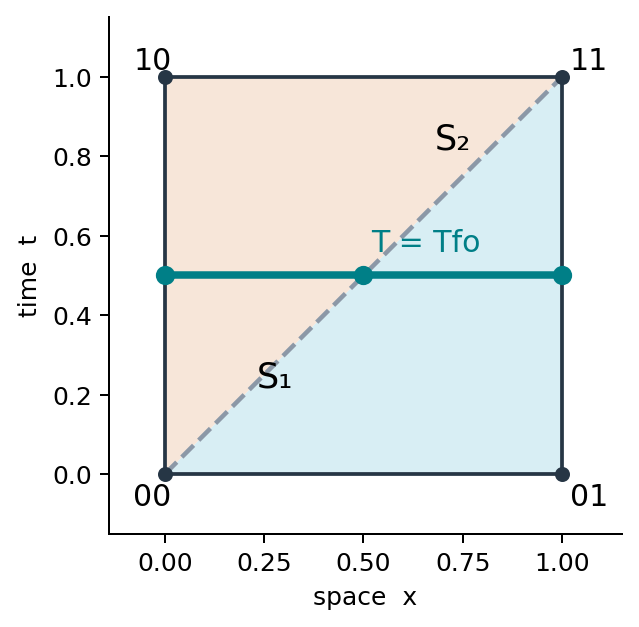
\includegraphics[width=0.68\textwidth,height=\textheight]{geometry_rectangle.png}
\caption{Two reference triangles and an example isothermal cut of a
spacetime rectangle}
\end{figure}

\subsubsection{3.2 Example in two spatial
dimensions}\label{example-in-two-spatial-dimensions}

One spacetime cube \((t,x,y)\in[0,1]^3\) has six tetrahedra, obtained by
permuting the coordinate order:

\begin{longtable}[]{@{}ll@{}}
\toprule\noalign{}
Increment order & Corner bit strings \\
\midrule\noalign{}
\endhead
\bottomrule\noalign{}
\endlastfoot
\(t,x,y\) & \(000,100,110,111\) \\
\(t,y,x\) & \(000,100,101,111\) \\
\(x,t,y\) & \(000,010,110,111\) \\
\(x,y,t\) & \(000,010,011,111\) \\
\(y,t,x\) & \(000,001,101,111\) \\
\(y,x,t\) & \(000,001,011,111\) \\
\end{longtable}

Each tetrahedron is checked separately. A one-hot/three-cold cut gives
one triangle. A two-hot/two-cold cut gives a quadrilateral, divided into
two triangles.

\begin{figure}
\centering
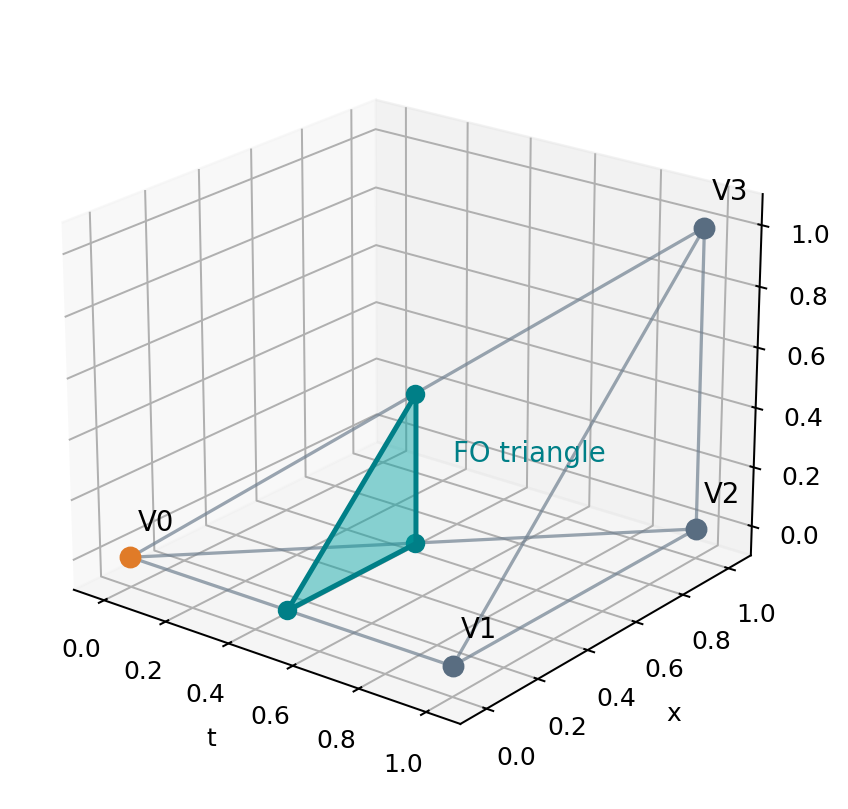
\includegraphics[width=0.7\textwidth,height=\textheight]{geometry_tetrahedron.png}
\caption{One reference tetrahedron and a freeze-out triangle for a
one-hot/three-cold configuration}
\end{figure}

\subsubsection{3.3 Example in three spatial
dimensions}\label{example-in-three-spatial-dimensions}

The 4D cell \((t,x,y,z)\in[0,1]^4\) has \(4!=24\) four-simplices. For
the order \((t,x,y,z)\), one is

\[
(0000,1000,1100,1110,1111).
\]

Every 4-simplex has five vertices and ten edges. An isotherm cuts it in
a \textbf{three-dimensional} polytope: either a tetrahedron (1-vs-4
signs) or a prism-like polytope (2-vs-3 signs), subdivided into three
freeze-out tetrahedra. The remaining 23 coordinate permutations are
constructed automatically, not hand-coded.

\subsection{4. Code map: what every component
represents}\label{code-map-what-every-component-represents}

The top-level structures in \texttt{SimplicialFreezeOut.jl} are:

\begin{Shaded}
\begin{Highlighting}[]
\KeywordTok{struct}\NormalTok{ RefSimplex\{D,C\}}
\NormalTok{    corners}\OperatorTok{::}\DataTypeTok{C                   }\CommentTok{\# D+1 bit{-}coded reference{-}cube corner IDs}
\NormalTok{    gradient\_map}\OperatorTok{::}\DataTypeTok{Matrix\{Float64\}  }\CommentTok{\# maps vertex temperature differences to grad\_s(T)}
\KeywordTok{end}

\KeywordTok{struct}\NormalTok{ ReferenceGrid\{D\}}
\NormalTok{    simplices}\OperatorTok{::}\DataTypeTok{Vector\{RefSimplex\{D\}\}}
\NormalTok{    cases}\OperatorTok{::}\DataTypeTok{Vector\{Vector\{NTuple\{D,Edge\}\}\}}
\KeywordTok{end}

\KeywordTok{struct}\NormalTok{ SurfaceElement\{D,F\}}
\NormalTok{    vertices}\OperatorTok{::}\DataTypeTok{NTuple\{D,NTuple\{D,Float64\}\}}
\NormalTok{    centroid}\OperatorTok{::}\DataTypeTok{NTuple\{D,Float64\}}
\NormalTok{    dsigma}\OperatorTok{::}\DataTypeTok{NTuple\{D,Float64\}}
\NormalTok{    fields}\OperatorTok{::}\DataTypeTok{F}
\KeywordTok{end}
\end{Highlighting}
\end{Shaded}

\texttt{RefSimplex} is an \textbf{input geometry object}.
\texttt{ReferenceGrid} holds all the precomputed input simplices and
sign-case topology. \texttt{SurfaceElement} is an \textbf{output
geometry object}: in \(D=4\) it contains four isothermal crossing points
forming one freeze-out tetrahedron.

The array \texttt{cases{[}mask+1{]}} contains \textbf{edge tuples}, not
positions; edge \((a,b)\) refers to local simplex vertices \(a,b\). The
points on these edges are evaluated at runtime.

\subsection{\texorpdfstring{5. Precomputation:
\texttt{\_reference\_simplices} and
\texttt{precompute}}{5. Precomputation: \_reference\_simplices and precompute}}\label{precomputation-_reference_simplices-and-precompute}

The function \texttt{\_permutations(collect(1:D))} enumerates the \(D!\)
coordinate orders. \texttt{\_reference\_simplices(Val(D))} walks from
\(0\) to \(1\) in each order, stores the bit-coded corner IDs, and
constructs

\[
B_{\mu a}=V_{a+1}^{\mu}-V_1^{\mu},\qquad a=1,\ldots,D.
\]

For an affine temperature \(T_h(s)=T_1+g_\mu(s^\mu-V_1^\mu)\), we have

\[
\begin{pmatrix}T_2-T_1\\ \vdots\\T_{D+1}-T_1\end{pmatrix}
=B^T g,
\qquad g=(B^T)^{-1}\Delta T.
\]

The code stores \texttt{(B\textquotesingle{})\^{}-1} in
\texttt{gradient\_map} \textbf{once}. On a physical cell, divide
\(g_\mu\) by the coordinate cell width \(h_\mu\) to recover
\(\partial T/\partial X^\mu\).

\texttt{precompute(Val(D))} then enumerates all hot/cold masks. There
are \(2^{D+1}\) possible assignments: 8, 16, and 32 in \(D=2,3,4\),
respectively.

\begin{Shaded}
\begin{Highlighting}[]
\NormalTok{reference }\OperatorTok{=} \FunctionTok{precompute}\NormalTok{(}\FunctionTok{Val}\NormalTok{(}\FloatTok{3}\NormalTok{))  }\CommentTok{\# D=3 {-}\textgreater{} 2 spatial dimensions, 6 tetrahedra}
\NormalTok{reference }\OperatorTok{=} \FunctionTok{precompute}\NormalTok{(}\FunctionTok{Val}\NormalTok{(}\FloatTok{4}\NormalTok{))  }\CommentTok{\# D=4 {-}\textgreater{} 3 spatial dimensions, 24 4{-}simplices}
\end{Highlighting}
\end{Shaded}

Compute \texttt{reference} once and reuse it across all cells and solver
steps.

\subsection{\texorpdfstring{6. Precomputing the intersection topology:
\texttt{\_case\_for\_mask}}{6. Precomputing the intersection topology: \_case\_for\_mask}}\label{precomputing-the-intersection-topology-_case_for_mask}

A temperature mask records only which vertices are hot. For \(D+1\)
vertices,

\[
\mathrm{mask}=\sum_{a=1}^{D+1}\mathbf1_{T_a\ge T_{\rm fo}}\,2^{a-1}.
\]

For \(D=3\), take local vertices 1,2 hot and 3,4 cold. There are four
hot-cold crossing edges:

\[
P_{00}=(1,3),\quad P_{01}=(1,4),\quad
P_{10}=(2,3),\quad P_{11}=(2,4).
\]

The intersection is a quadrilateral; the precomputed two-triangle
pattern is

\[
(P_{00},P_{01},P_{11}),\qquad(P_{00},P_{11},P_{10}).
\]

The symbols \(P_{ij}\) here are \textbf{names of edges}. They do not
become points until we insert actual temperatures.

For \(D=4\), take local vertices 1,2 hot and 3,4,5 cold. Six crossing
edges form a prism. Define \(A_i=(1,i+3)\) and \(B_i=(2,i+3)\) for
\(i=0,1,2\). Three output tetrahedra are:

\[
(A_0,A_1,A_2,B_2),\quad
(A_0,A_1,B_1,B_2),\quad
(A_0,B_0,B_1,B_2).
\]

This convention fixes the prism diagonals. Face conformity should be
checked when combining neighboring simplices, particularly in degenerate
cases.

\subsection{7. Runtime: from one grid cell to actual crossing
points}\label{runtime-from-one-grid-cell-to-actual-crossing-points}

The central function is

\begin{Shaded}
\begin{Highlighting}[]
\FunctionTok{extract\_isosurface}\NormalTok{(temperature, axes, Tfo;}
\NormalTok{    fields}\OperatorTok{=}\FunctionTok{NamedTuple}\NormalTok{(), reference}\OperatorTok{=}\FunctionTok{precompute}\NormalTok{(}\FunctionTok{Val}\NormalTok{(}\FunctionTok{ndims}\NormalTok{(temperature))))}
\end{Highlighting}
\end{Shaded}

The first array dimension is time. \texttt{axes} is a tuple of strictly
increasing physical coordinate arrays. A 2+1D example uses
\texttt{T{[}it,ix,iy{]}} and \texttt{(t,x,y)}; 3+1D uses
\texttt{T{[}it,ix,iy,iz{]}} and \texttt{(t,x,y,z)}.

The outer loop visits spacetime cells. For each cell, \texttt{lows}
holds the low coordinate of every axis and \texttt{widths} its size;
\texttt{corner\_temp} stores all \(2^D\) corner temperatures. If the
entire cell is above or below \(T_{\rm fo}\), it can be skipped
immediately.

Otherwise, the program iterates over \textbf{all} reference simplices of
that cell:

\begin{Shaded}
\begin{Highlighting}[]
\ControlFlowTok{for}\NormalTok{ template }\KeywordTok{in}\NormalTok{ reference.simplices}
\NormalTok{    Tverts }\OperatorTok{=} \FunctionTok{ntuple}\NormalTok{(a }\OperatorTok{{-}\textgreater{}}\NormalTok{ corner\_temp[template.corners[a]], D}\OperatorTok{+}\FloatTok{1}\NormalTok{)}
\NormalTok{    mask }\OperatorTok{=} \FunctionTok{sum}\NormalTok{((Tverts[a] }\OperatorTok{\textgreater{}=}\NormalTok{ Tfo ? }\FloatTok{1} \OperatorTok{:} \FloatTok{0}\NormalTok{) }\OperatorTok{\textless{}\textless{}}\NormalTok{ (a}\OperatorTok{{-}}\FloatTok{1}\NormalTok{) }\ControlFlowTok{for}\NormalTok{ a }\KeywordTok{in} \FloatTok{1}\OperatorTok{:}\NormalTok{D}\OperatorTok{+}\FloatTok{1}\NormalTok{)}
\NormalTok{    patterns }\OperatorTok{=}\NormalTok{ reference.cases[mask}\OperatorTok{+}\FloatTok{1}\NormalTok{]}
    \FunctionTok{isempty}\NormalTok{(patterns) }\OperatorTok{\&\&} \ControlFlowTok{continue}
    \CommentTok{\# Locate the crossing on each edge of every output surface element.}
\ControlFlowTok{end}
\end{Highlighting}
\end{Shaded}

For edge \((a,b)\) with opposite signs, calculate

\[
\theta_{ab}=\frac{T_{\rm fo}-T_a}{T_b-T_a},\qquad
Y_{ab}=X_a+\theta_{ab}(X_b-X_a).
\]

This is the \textbf{only geometric interpolation used in the
piecewise-linear algorithm}. The point \(Y_{ab}\) lies on the isotherm
of the affine temperature field.

Inside a cell, the normalized reference coordinate \(s\) is converted to
physical coordinates through \(X^\mu=L^\mu+h_\mu s^\mu\). This works on
nonuniform Cartesian-product axes because each cell has its own widths.

\subsection{8. Worked 2+1D example, with actual
numbers}\label{worked-21d-example-with-actual-numbers}

Consider one reference tetrahedron

\[
V_1=(0,0,0),\ V_2=(1,0,0),\ V_3=(1,1,0),\ V_4=(1,1,1).
\]

Let the signed temperatures \(F_a=T_a-T_{\rm fo}\) be

\[
(F_1,F_2,F_3,F_4)=(0.6,0.2,-0.4,-0.2).
\]

Vertices 1,2 are hot; 3,4 are cold. Four edges cross the isotherm. Their
crossing fractions are

\[
\theta_{13}=0.6/(0.6+0.4)=0.6,\quad
\theta_{14}=0.6/(0.6+0.2)=0.75,
\]

\[
\theta_{23}=0.2/(0.2+0.4)=1/3,\quad
\theta_{24}=0.2/(0.2+0.2)=1/2.
\]

Thus the intersection points are

\[
P_{13}=(0.6,0.6,0),\quad P_{14}=(0.75,0.75,0.75),
\] \[
P_{23}=(1,1/3,0),\quad P_{24}=(1,1/2,1/2).
\]

The quadrilateral \((P_{13},P_{14},P_{24},P_{23})\) is divided into two
triangles. Their oriented area covectors will be computed and summed. No
global point sorting or spline fitting is needed.

\textbf{Simplest planar test.} Let \(F=\tfrac12-t\) on a unit cube. The
six spacetime tetrahedra together reconstruct the plane \(t=\tfrac12\).
The sum over all freeze-out triangles satisfies

\[
\sum_{K}\Delta\sigma_{\mu,K}=(1,0,0),
\]

because the hot region is at \(t<1/2\). The analogous one-cell result is
\((1,0)\) for \(D=2\) and \((1,0,0,0)\) for \(D=4\).

\subsection{\texorpdfstring{9. Computing and orienting \texttt{dsigma}:
\texttt{\_area\_covector}}{9. Computing and orienting dsigma: \_area\_covector}}\label{computing-and-orienting-dsigma-_area_covector}

Each output surface \((D-1)\)-simplex has \textbf{D} vertices
\(Y_1,\ldots,Y_D\) and \(D-1\) tangent edges \(e_a=Y_{a+1}-Y_1\). The
integrated coordinate-oriented hypersurface covector is

\[
\boxed{\displaystyle
\Delta\sigma_\mu=\frac1{(D-1)!}
\epsilon_{\mu\nu_1\cdots\nu_{D-1}}
 e_1^{\nu_1}\cdots e_{D-1}^{\nu_{D-1}}.}
\]

The code computes these components through signed determinants of the
\((D-1)\times(D-1)\) minors of the tangent matrix. The initial sign
depends on how the vertices were ordered.

An affine temperature has a constant coordinate gradient
\(g_\mu=\partial_\mu T_h\) within the input spacetime simplex. The code
flips the output orientation, if needed, to have

\[
\sum_\mu\Delta\sigma_\mu g_\mu\le0,
\]

where this last dot product is used \textbf{only as a coordinate-based
sign test}, not as a Lorentzian contraction. In words, the
coordinate-oriented hypersurface covector points toward colder
temperature.

To convert a coordinate hypersurface element to the physical one in
Milne coordinates, include \(\sqrt{-g}=\tau\) in the \textbf{quadrature
measure}. The module's \texttt{dsigma} does not include this factor.

\subsection{10. Interpolating hydrodynamic fields at the
centroid}\label{interpolating-hydrodynamic-fields-at-the-centroid}

The output geometry has a centroid \(X_c=\frac1D\sum_{k=1}^{D}Y_k\). A
scalar or vector field is reconstructed affinely from the original
spacetime simplex corners, using barycentric weights.

If \(Y_k=(1-\theta_k)V_{a_k}+\theta_kV_{b_k}\), the centroid weights are

\[
w_a=\frac1D\sum_{k=1}^D\big[(1-\theta_k)\mathbf1_{a=a_k}
+\theta_k\mathbf1_{a=b_k}\big].
\]

Then \(q(X_c)=\sum_a w_a q(V_a)\) for an affine field. In the code,
\texttt{weights} is accumulated within the edge-crossing loop;
\texttt{\_fields\_at\_centroid} applies the same weights to each
supplied array. The surface temperature itself is not returned among
\texttt{fields} unless it is explicitly supplied.

The centroid is only a quadrature approximation for nonlinear
Cooper--Frye integrands. Additional surface quadrature points can be
added later, while retaining exactly the same topology.

\subsection{\texorpdfstring{11. \texttt{integrate\_surface}: geometry
versus
physics}{11. integrate\_surface: geometry versus physics}}\label{integrate_surface-geometry-versus-physics}

\begin{Shaded}
\begin{Highlighting}[]
\FunctionTok{integrate\_surface}\NormalTok{(elements,}
    \ConstantTok{e} \OperatorTok{{-}\textgreater{}} \FunctionTok{sum}\NormalTok{(J[mu]}\OperatorTok{*}\ConstantTok{e}\NormalTok{.dsigma[mu] }\ControlFlowTok{for}\NormalTok{ mu }\KeywordTok{in} \FloatTok{1}\OperatorTok{:}\NormalTok{D);}
\NormalTok{    measure }\OperatorTok{=}\NormalTok{ x }\OperatorTok{{-}\textgreater{}} \FloatTok{1.0}\NormalTok{)}
\end{Highlighting}
\end{Shaded}

Here \texttt{e.dsigma} is an \textbf{integrated coordinate area
covector}, so do \textbf{not} multiply again by the segment length,
triangle area, or tetrahedron volume. The function \texttt{integrand(e)}
should contract a current with \texttt{e.dsigma} and use
\texttt{e.fields} as needed. \texttt{measure(x)} is the coordinate
metric-volume density, e.g.~\texttt{x\ -\textgreater{}\ x{[}1{]}} for
Milne coordinates when the first coordinate is \(\tau\).

For particle spectra, \(p^\mu\Delta\sigma_\mu f(X_c,p)\) is multiplied
by the correct phase-space normalization, quantum distribution, viscous
corrections, and metric factor. Those physical factors are deliberately
outside this geometry-only module.

\subsection{12. How to run the code, step by
step}\label{how-to-run-the-code-step-by-step}

\begin{Shaded}
\begin{Highlighting}[]
\ExtensionTok{julia}\NormalTok{ walkthrough.jl                 }\CommentTok{\# explains all D=2,3,4 reference cases}
\ExtensionTok{julia}\NormalTok{ demo.jl                        }\CommentTok{\# example smooth temperature profiles}
\ExtensionTok{julia}\NormalTok{ test\_simplicial\_freezeout.jl   }\CommentTok{\# built{-}in geometry checks}
\end{Highlighting}
\end{Shaded}

In \texttt{walkthrough.jl}, a single unit cell is filled with
\(T(t)=1.5-t\), with \(T_{\rm fo}=1\). The exact isotherm is \(t=0.5\).
It prints every simplex, its hot/cold mask, the number of output pieces,
and checks the sum of the oriented hypersurface vectors against
\((1,0,\ldots,0)\). The test also samples an affine scalar field at
surface centroids.

To use a real grid, call

\begin{Shaded}
\begin{Highlighting}[]
\FunctionTok{include}\NormalTok{(}\StringTok{"SimplicialFreezeOut.jl"}\NormalTok{)}
\ImportTok{using} \BuiltInTok{.SimplicialFreezeOut}

\NormalTok{ref }\OperatorTok{=} \FunctionTok{precompute}\NormalTok{(}\FunctionTok{Val}\NormalTok{(}\FloatTok{4}\NormalTok{))}
\NormalTok{surface }\OperatorTok{=} \FunctionTok{extract\_isosurface}\NormalTok{(T, (t,x,y,z), Tfo;}
\NormalTok{    fields}\OperatorTok{=}\NormalTok{(ux}\OperatorTok{=}\NormalTok{ux, uy}\OperatorTok{=}\NormalTok{uy, uz}\OperatorTok{=}\NormalTok{uz), reference}\OperatorTok{=}\NormalTok{ref)}

\ControlFlowTok{for} \ConstantTok{e} \KeywordTok{in}\NormalTok{ surface}
\NormalTok{    X }\OperatorTok{=} \ConstantTok{e}\NormalTok{.centroid       }\CommentTok{\# (t,x,y,z)}
\NormalTok{    normal\_area }\OperatorTok{=} \ConstantTok{e}\NormalTok{.dsigma  }\CommentTok{\# coordinate{-}area covector}
\NormalTok{    u }\OperatorTok{=} \ConstantTok{e}\NormalTok{.fields         }\CommentTok{\# sampled velocity components}
\ControlFlowTok{end}
\end{Highlighting}
\end{Shaded}

If a method-of-lines integrator generates time slices sequentially, pass
an array with only two consecutive time slices (shape
\((2,n_x,n_y,n_z)\)) and their two time coordinates. Repeat on each time
interval and append the results. This can avoid storing the full
evolution in RAM.

\subsection{13. Checks, limitations, and next
improvements}\label{checks-limitations-and-next-improvements}

\textbf{Geometry tests.} First test a planar field
\(F(X)=a_\mu X^\mu-b\); every crossing point should satisfy \(F=0\) to
roundoff, and the oriented total should have the expected sign and
magnitude. A closed polyhedral boundary should have vanishing total
integrated coordinate area covector. The freeze-out surface alone need
not be closed: initial/final and outer-domain pieces matter for a
conservation test.

\textbf{Degenerate cases.} Equality \(T_a=T_{\rm fo}\) is assigned to
the hot side in the module; zero-area elements are discarded.
Exactly-on-surface edges, vertices, and entire plateaus require special
treatment in production software.

\textbf{Accuracy.} The interpolation is affine inside each input
simplex. Refining only Cooper--Frye quadrature does not correct the
geometry. The simplex subdivision can produce mesh-direction bias and
should be checked against rotated analytic profiles or CORNELIUS.

\textbf{Time accuracy.} Although a method-of-lines solver may have a
high-order time interpolant, this version uses only the supplied sampled
time slices and linear interpolation in time. A future implementation
could evaluate temperature at additional time nodes or use higher-order
local reconstruction.

\textbf{Memory and performance.} This is a readable reference
implementation. It allocates matrices for the small cofactors and stores
all surface elements. Production Julia code should consider
\texttt{StaticArrays}, allocation-free determinant formulas for
\(D\le4\), cached shared-edge crossing points, and streaming
accumulation of quadrature contributions.

\textbf{Validation status.} The Julia code is supplied with executable
tests, but a Julia runtime is not available in this environment;
numerical equivalence and performance must be checked with a local Julia
installation.

\subsubsection{One-sentence summary}\label{one-sentence-summary}

\textbf{The grid fixes which spacetime simplices exist; the temperature
fixes which edges cross; the lookup table fixes how the crossings
connect; the determinants supply the oriented surface elements.}

\end{document}
